
\begin{figure}[H]
	\centering    
          \begin{tikzpicture}[->,>=stealth',shorten >=1pt,auto,node distance=.45cm,
  thick,main node/.style={observed}, hidden/.style={empty},background rectangle/.style={fill=olive!45}]
%every node/.style={scale=0.6}
 %nodes
\node[main node](1){$X_{1}$};
\node[main node, right=of 1](2){$X_{2}$};
\node[hidden, right=of 2](3){$...$};
\node[main node, right=of 3](4){$X_{N}$};
\node[main node, below right=of 2](5){$Y$};
\node[main node, above right=of 2](6){$Z$};
 \path[every node/.style={font=\tiny}]
    (1) edge (5)
    	(2) edge (5)
    (4) edge (5)
    (6) edge (1) edge (2) edge (4);
\end{tikzpicture}
        \caption{Confounded graph}
        \label{fig:parallel_confounded} 
\end{figure}


We now compare the general algorithm with a range of standard bandit algorithms on the confounded graph in Figure \ref{fig:parallel_confounded}. All the variables are binary and the action space consists of the set of single variable interventions plus the do nothing action, $\calA = \set{\set{do(X_i = j)} \cup \set{do(Z = j)} \cup \set{do()}: 1\leq i \leq N,\; j \in \set{0,1}}$. We choose this setting because it generalises the parallel bandit, while simultaneously being sufficiently simple that we can compute the exact reward and interventional distributions for large $N$ (in general inference in graphical models is exponential in $N$). As before, we show the average regret over 10,000 simulations with error bars showing three standard errors. 

In Figure \ref{fig:simple_vs_m_general} we fix $N$ and $T$ and $P(Z=1) = .4$. For some $2 \leq N_1 \leq N$ we define 
\eq{
P(X_i = 1|Z = 0) &= \begin{cases} 0 & \text{ if } i \in \set{1,...N_1} \\ .4 & \text{ otherwise } \end{cases}\\
P(X_i = 1|Z = 1) &= \begin{cases} 0 & \text{ if } i \in \set{1,...N_1} \\ .65 & \text{ otherwise } \end{cases}
}
As in the parallel bandit case, we let $Y$ depend only on $X_1$, $P(Y|do(X_1=1)) = \frac{1}{2} + \epsilon$ and $P(Y|do(X_1=0)) = \frac{1}{2}-\epsilon'$, where $\epsilon' = \epsilon P(X_1=1) / P(X_1=0)$. The value of $N_1$ determines $m$ and ranges between $2$ and $N$. The values for the CPD's have been chosen such that the reward distribution is independent of $m$ and so that we can analytically calculate $\eta*$. This allows us to just show the dependence on $m$, removing the noise associated with different models selecting values for $\eta*$ with the same $m$ (and also worst case performance), but different performance for a given reward distribution. 

In Figure \ref{fig:simple_vs_T_general} we fix the model and number of variables, $N$, and vary the horizon $T$. $P(Z)$ and $P(X|Z)$ are the same as for the previous experiment.  
In Figure \ref{fig:simple_vs_T_misspecified} we additionally show the performance of Algorithm 1, but exclude actions on $Z$ from the set of allowable actions to demonstrate that Algorithm 1 can fail in the presence of a confounding variable, which occurs because it incorrectly assumes that $P(Y|do(X)) = P(Y|X)$. 
We let $P(Z) = .6$, $P(Y|\boldsymbol{X}) = X_7 \oplus X_N$ and $P(X|Z)$ be given by:

\eq{
P(X_i = 1|Z = 0) &= 
\begin{cases} 
.166 & \text{ if } i \in \set{1,..., 6} \\
.2 & \text{ if } i = 7 \\
.7 & \text { otherwise} 
 \end{cases}\\
 P(X_i = 1|Z = 1) &= 
\begin{cases} 
.166 & \text{ if } i \in \set{1,..., 6} \\
.8 & \text{ if } i = 7 \\
.3 & \text { otherwise} 
 \end{cases}\\
}

In this setting $X_7$ tends to agree with $Z$ and $X_N$ tends to disagree. It is sub-optimal to act on either $X_7$ or $X_N$, while all other actions are optimal. The first group of $X$ variables with $i \leq 6$ will be identified by the parallel bandit as the most unbalanced ones and played explicitly. All remaining variables are likely to be identified as balanced and estimated from observational estimates. The CPD values have been chosen to demonstrate the worst case outcome, where the bias in the estimates leads Algorithm 1 to asymptotically select a sub-optimal action.

\begin{figure}[H]
    \begin{subfigure}[t]{0.3\textwidth}
		\centering    
    		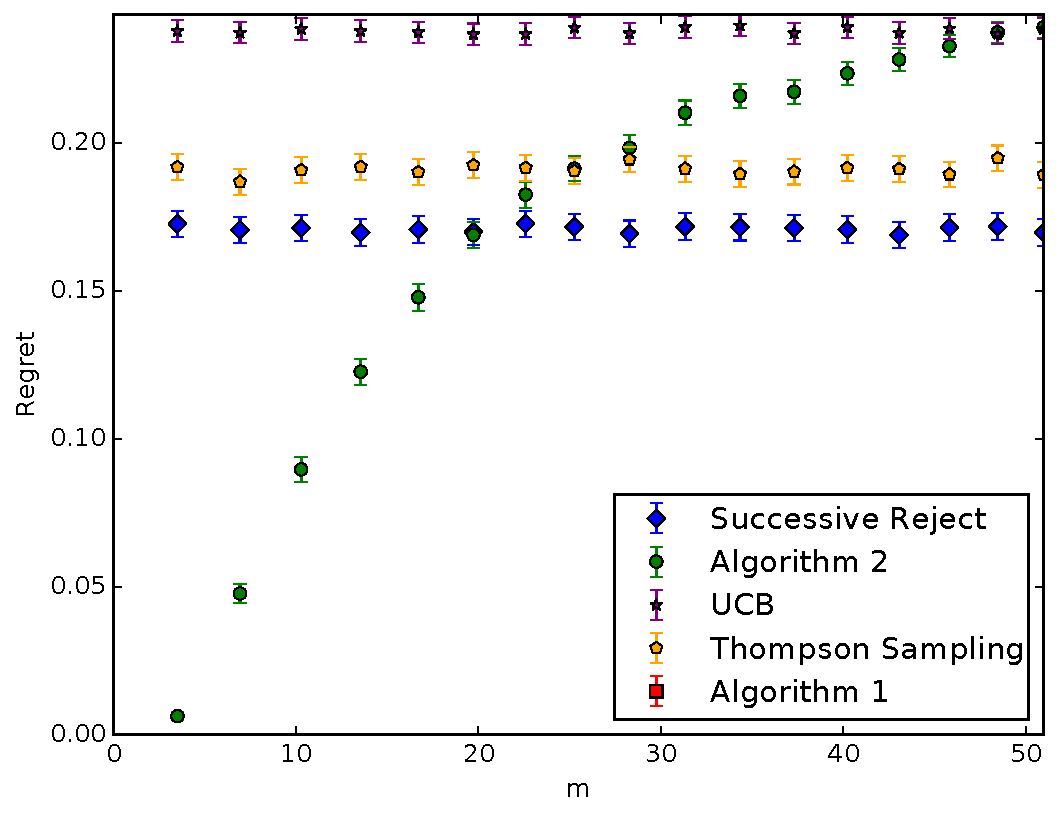
\includegraphics[width=\textwidth]{experiment4_20161023_2120.pdf}
    		\caption{Simple regret vs $m(\eta*)$ for fixed horizon $T=400$ and number of variables $N = 50$}
        \label{fig:simple_vs_m_general}
    \end{subfigure}\hfill
    \begin{subfigure}[t]{0.3\textwidth}
    		\centering
        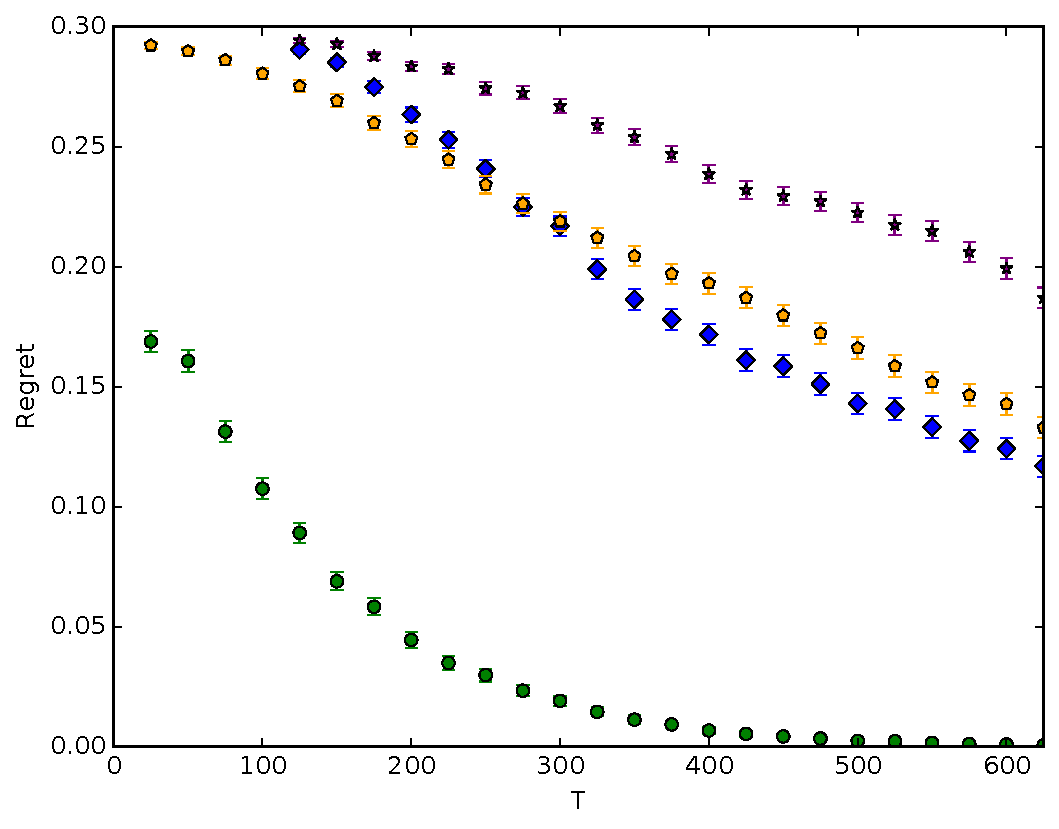
\includegraphics[width=\textwidth]{experiment7_20161020_1257.pdf}
    		\caption{Simple regret vs horizon, $T$, with $N = 50$ and $m(\eta*)=3.1$ }
        \label{fig:simple_vs_T_general}
    \end{subfigure}\hfill
    \begin{subfigure}[t]{0.3\textwidth}
    		\centering
    		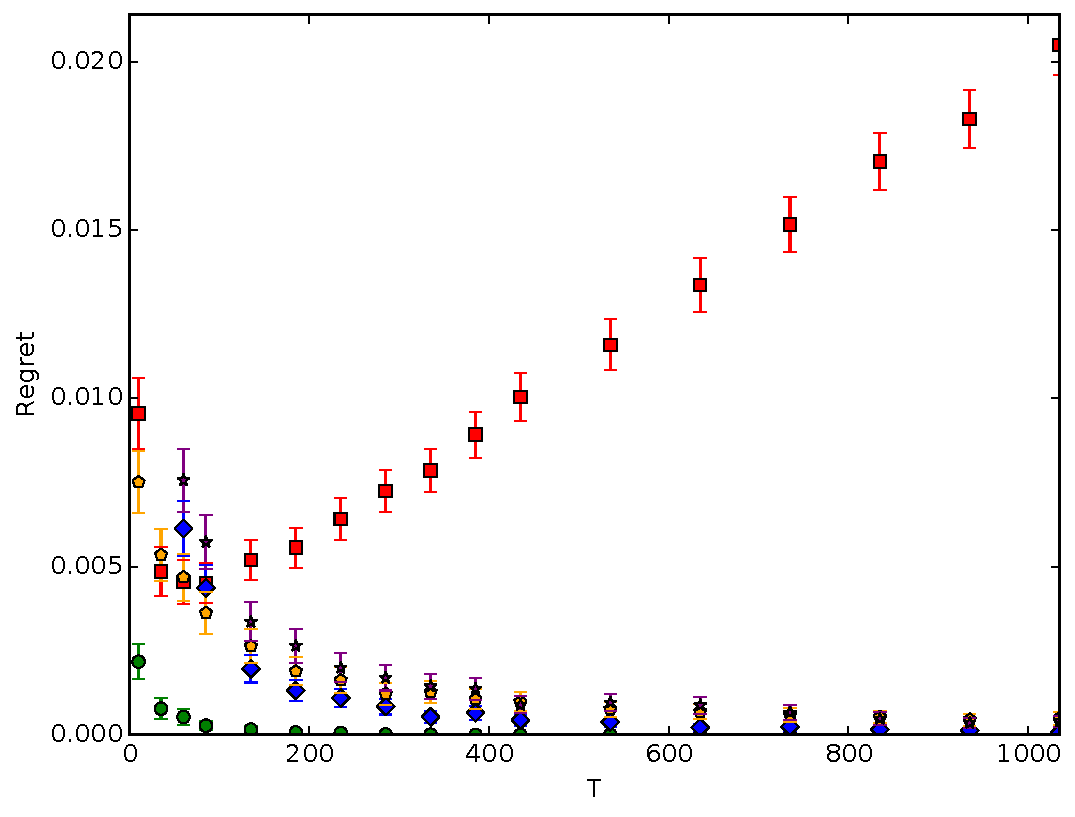
\includegraphics[width=\textwidth]{experiment5_20161023_2118.pdf}
    		\caption{Simple regret vs horizon, $T$, with $N = 21$, $m(\eta*)=4.3$ with no actions setting $Z$}
    		\label{fig:simple_vs_T_misspecified}
    \end{subfigure}
    \caption{Experimental results on the confounded graph}
    \label{fig:experiments_confounded}
\end{figure}


